% !TEX root = ../thesis.tex
\chapter{Data Collection}
\label{capitolo3}
\thispagestyle{empty}


In this chapter we will present all the available datasets containing bot accounts, with all the tools and methodologies used to collect new data. The final dataset contains:

\begin{itemize}
\item[\PencilRight]
Data from existing datasets
\item[\PencilRight]
Data collected with different approaches
\item[\PencilRight]
Hand-labeled data
\end{itemize}



\section{Tools}
Different tools were used in order to both collect the data and to enrich existing ones. This stage was essential to gather additional features. Here we present all the instruments involved in this section.

\subsection{Tweepy}
Tweepy is a python wrapper for the Twitter API.
Two main methods were used to collect all the dafault features of users and tweets:\\

\begin{tabular}{ccc}
\centering	
	Method&Input&Output\\ \hline\hline
	API.get\_user&[id/user\_id/screen\_name]&User object\\
	API.user\_timeline&[user\_id][, count]&list of Status object\\ \hline\\
\end{tabular}

A User object contains all that features that describe the user's profile and his utilization of Twitter.
A Status object contains the datails of a single tweet, such as the full text, number of retweets and replies.

\subsection{Botometer}
Botometer (https://botometer.iuni.iu.edu) checks the activity of a Twitter account and gives it a score based on how likely the account is to be a bot.
Using their dataset they tested most classification algorithm and highlighted Random Forest as their final classifier, since it gained the highest accuracy. Its accuracy was 98.42\% and 0.984 F1 measure\cite{Lee11sevenmonths}.
\\Botometer provides API to check Twitter accounts genuinity.

\subsection{Hoaxy}
Hoaxy is a tool that visualizes the spread of articles online. Articles can be found on Twitter, or in a corpus of claims and related fact checking. 
Hoaxy only checks the news sources and compares them with a list of unreliable URLs.

\section{Datasets}

\subsection{Caverlee-2011}
This dataset is composed by content polluters, detected by a social honeypot, and legitimate users sampled from Twitter.
For each content polluter, they save their 200 most recent tweets, their following and follower graph, and the temporal and historical profile informations.
In order to collect genuine users, they randomly sampled about 20.000 Twitter ids and monitored them for three months, to see if they were still active and not suspended by the social platform moderation service.\cite{Lee11sevenmonths}.


\subsection{Cresci-2017}
Cresci Dataset is composed by genuine accounts and bots. In this dataset there is a deeper differentiation for the bots, which are precisely labeled according to different categories.

\tiny
\begin{center}
\begin{tabular}{ccccc}
	Dataset&Description&\#Users&\#Tweets&Year\\ \hline\hline
	genuine accounts&
	verified accounts that are human-operated&
	3,474&
	8,377,522
	&2011\\
	social spambots \#1&
	retweeters of an Italian political candidate&
	991&
	1,610,176&
	2012 \\
	social spambots \#2&
	spammers of paid apps for mobile devices&
	3,457&
	428,542&
	2014 \\
	social spambots \#3&
	spammers of products on sale at	Amazon&
	464&
	1,418,626&
	2011 \\
	traditional spambots \#1&
	training set of spammers used by Yang\cite{Yang}&
	1,000&
	145,094&
	2009 \\
	traditional spambots \#2&
	spammers of scam URLs&
	100&
	74,957&
	2014 \\
	traditional spambots \#3&
	automated accounts spamming job offers&
	433&
	5,794,931&
	2013 \\
	traditional spambots \#4&
	automated accounts spamming job offers&
	1,128&
	133,311&
	2009 \\
	fake followers&
	accounts inflating followers of other accounts&
	3,351&
	196,027&
	2012 \\ \hline\\
	
\end{tabular}
\end{center}

\normalsize
\begin{itemize}
	\item \textbf{Genuine accounts} are those users who correctly answered to a simple question, posed in natural language, so they represent accounts with no automatization.
	\item  During Rome majoral election in 2014, one of the candidates used a set of automated accounts to publicize his policies. These accounts were gathered to be part of the \textbf{Social spambots \#1}.
	\item \textbf{Social spambots \#2} are accounts that promotes mobile app, using popular hashtags for months.
	\item  \textbf{Social spambots \#3} promotes products on sale on Amazon, by tweeting products URL and descriptions.
\end{itemize}


All these accounts were manually checked to verify their automated nature.

\begin{itemize}
	\item The \textbf{Traditional spambots \#1} dataset is the training set used in \cite{Yang}.
	\item \textbf{traditional spambots \#2} are users that mention other users in tweets containing scam URLs. They usually invite users to claim a prize.
	\item  \textbf{Traditional spambots \#3} and \textbf{traditional spambots \#4} are bots that continously tweet job offers.
	\item \textbf{Fake followers} are account involved in increasing popularity of other users. In order to collect them, they bought followers from fastfollowerz.com, intertwitter.com and twittertechnology.com. \cite{Cresci}
\end{itemize}


\subsection{Varol-2017}
This dataset contains a list of Twitter accounts, labeled as bots (1) or humans (0). 
The construction of the Varol dataset starts with the indentification of a representative sample of users, by monitoring a Twitter stream for 3 months, starting in October 2015. Thanks to this approach it is possible to collect data without bias; in fact other methods like snowball or breadth-first need an initial users set.
During the observation window about 14 million user accounts has been gathered. 
All the collected users must have at least 200 tweets in total and 90 tweets during the three month observation (about one tweet per day).
\\
Using the classifier trained on the honeypot dataset in \cite{Lee11sevenmonths}, they computed the classification scores for each of the active accounts. 
Then the samples were grouped by their score and 300 accounts from each bot-score decile were randomly selected. 
The 3000 extracted accounts were manually labeled by some volunteers. They analyzed users profile, friends, tweets, retweets and interactions with other users. Then they assingned a label to each user.
Of course the final decision is conditioned to personal opinion\cite{Varol}.

\subsection{BotBlock}
Botblock (https://github.com/dansarie/Botblock) is a Twitter block list containing the user ids of a large number of known porn bot accounts. They are mainly used to aggressively market porn sites.

\section{Varol clustering}
As a first try, we wanted to undestand if different kinds of bots were easy to distinguish, using their profile features only. Moreover, we didn't know what kinds of bots populate Twitter for the most. So an unsuperised approach could have helped us to define different categories. We relied expectations on clustering techniques, hoping to get a solid help in automatizing the labeling process of the data.
We used the Varol dataset\cite{Varol}, that contains a plain list of bots and humans.
It was not possible to use all the data, because we need to scrape from the web all the possible features. Some of the listed accounts was deleted, so for this work we could use only those accounts that was still active.
The first step was the knee-elbow analisys based on a hierarchical clustering with single linkage and euclidean distance. The data must had been preprocessed and cleaned.
Here we illustrate what kind of preprocess operations have been performed:

\small
\begin{center}
	\begin{tabular}{ccc}
		\\feature&type&preprocess operation\\
		\hline\hline
		id&int&delete\\
		name&str&replace with len(name)\\
		screen\_name&str&replace with len(screen\_name)\\
		statuses\_count&int&/\\
		followers\_count&int&/\\
		friends\_count&int&/\\
		favourites\_count&int&/\\
		listed\_count&int&/\\
		url&str&replace with hasUrl (0/1)\\
		lang&str&one hot encoding\\
		time\_zone&str&one hot encoding\\
		location&str&one hot encoding\\
		default\_profile&int&replace with hasDefaultProfile (0/1)\\
		default\_profile\_image&boolean&boolean to int (0/1)\\
		geo\_enabled&boolean&boolean to int (0/1)\\
		profile\_image\_url&str&delete\\
		profile\_use\_background\_image&boolean&boolean to int (0/1)\\
		profile\_background\_image\_url\_https&str&delete\\
		profile\_text\_color&str&delete\\
		profile\_image\_url\_https&str&delete\\
		profile\_sidebar\_border\_color&str&delete\\
		profile\_background\_tile&boolean&boolean to int (0/1)\\
		profile\_sidebar\_fill\_color&str&delete\\
		profile\_background\_image\_url&str&delete\\
		profile\_background\_color&str&delete\\
		profile\_link\_color&str&delete\\
		utc\_offset&int&delete\\
		is\_translator&boolean&boolean to int (0/1)\\
		follow\_request\_sent&int&delete\\
		protected&boolean&boolean to int (0/1)\\
		verified&boolean&boolean to int (0/1)\\
		notifications&boolean&delete\\
		description&str&replace with hasDescription (0/1)\\
		contributors\_enabled&boolean&boolean to int (0/1)\\
		following&boolean&delete\\
		created\_at&str&string to int (year)\\\hline\\
	\end{tabular}
\end{center}

\normalsize
\clearpage

Since we didn't know how many categories of bots have been included in this dataset, the first step consists in understand how many clusters represents the optimal solution. To perform this task, we applied \textit{hierarchical clustering}. In figure (\ref{fig:dendogram}) you can see the dendogram of the algorithm.


\begin{figure}
	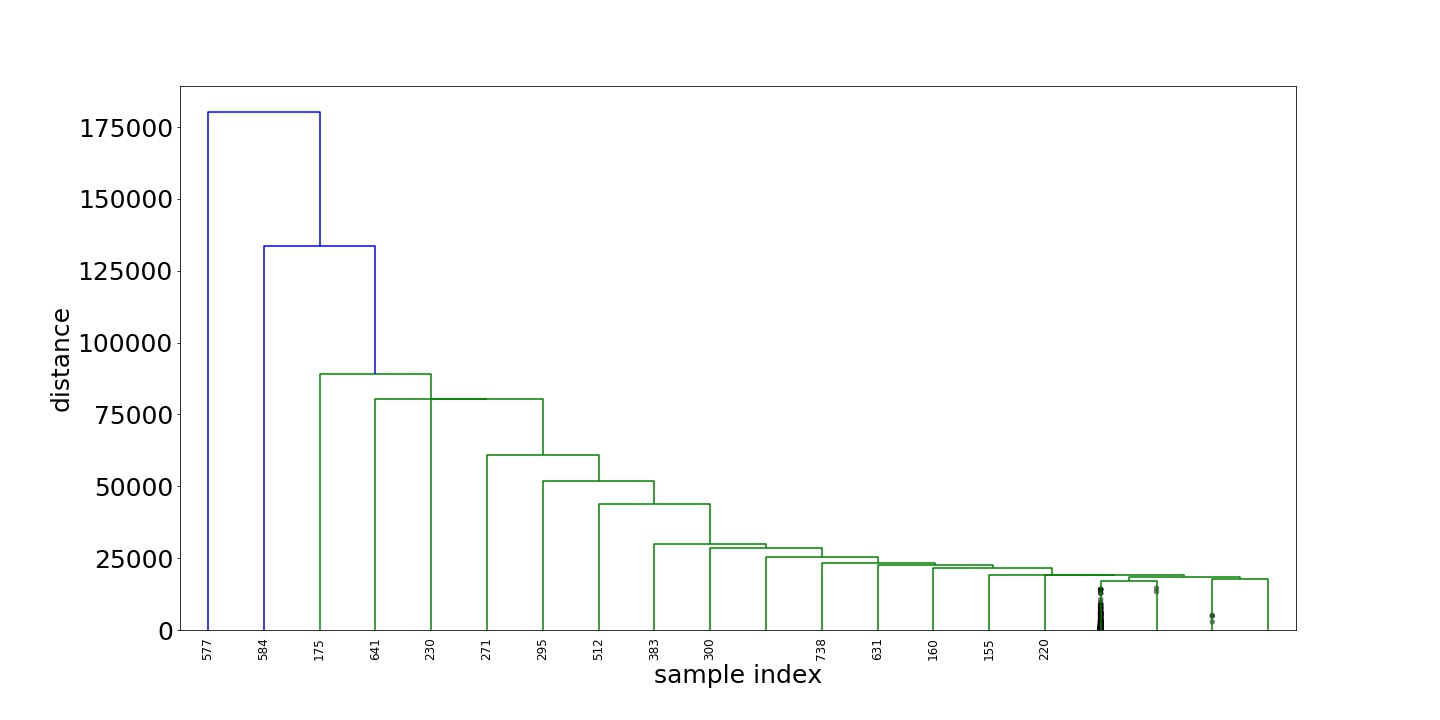
\includegraphics[width=\linewidth]{chapter3/figure/dendogram.jpg}
	\caption{Hierarchical Clustering Dendrogram (truncated to the last 20 merged clusters)}
	\label{fig:dendogram}
\end{figure}

In order to select the optimal number of clusters, we plotted the knee-elbow figure (\ref{fig:kneeelbow}). It shows the variation of WSS (within cluster sum of squares) and BSS (between cluster sum of squares) as the number of clusters increase.
It is clear that there are no well-defined elbows or knees, both curves seems to be "smooth", so it is not possible to choose a reasonable k.

\begin{figure}
	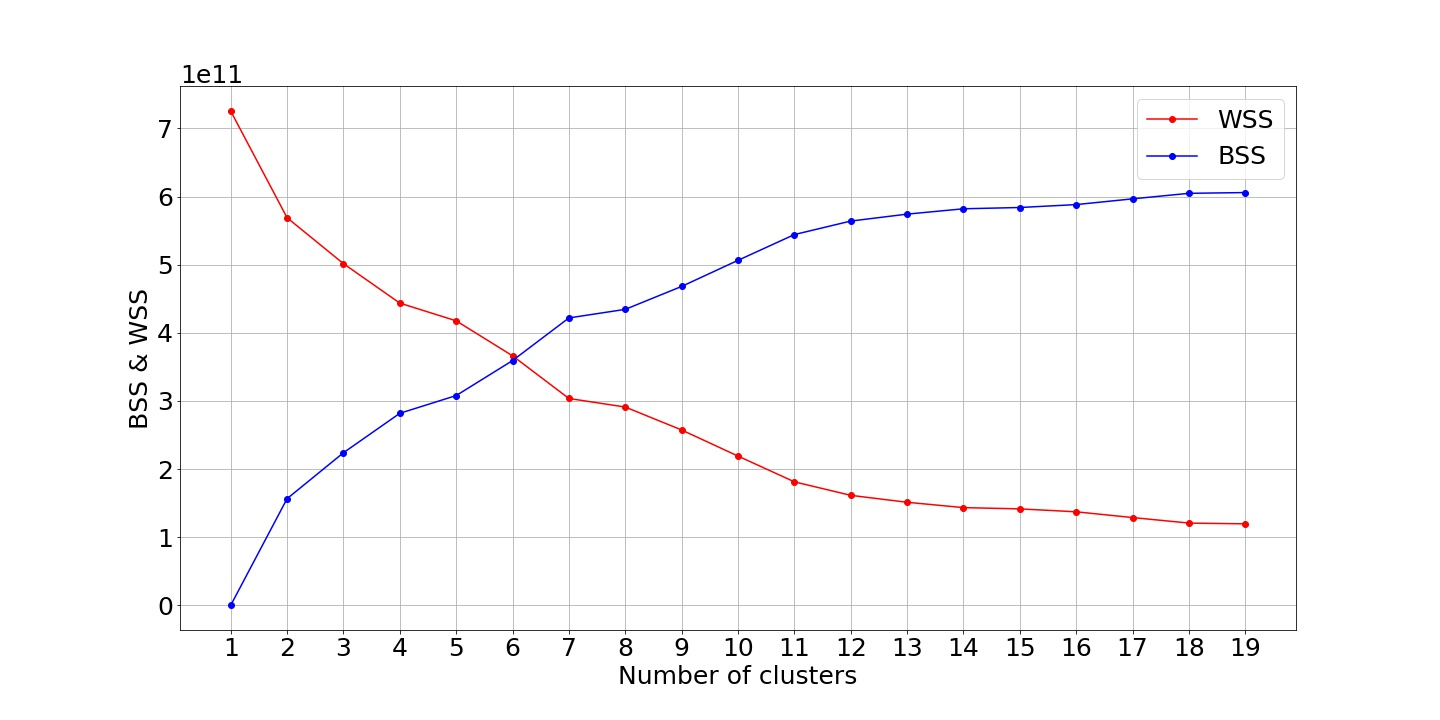
\includegraphics[width=\linewidth]{chapter3/figure/kneeelbow.jpg}
	\caption{Hierarchical Clustering - knee-elbow}
	\label{fig:kneeelbow}
\end{figure}

Then we tried another approach. We applied the \textit{K-means} algorithm and we plotted the elbow methond (\ref{fig:elbow}). In this figure there is an elbow beetween k=3 and k=4, so the most accurate solution is to select 4 clusters.

\begin{figure}
	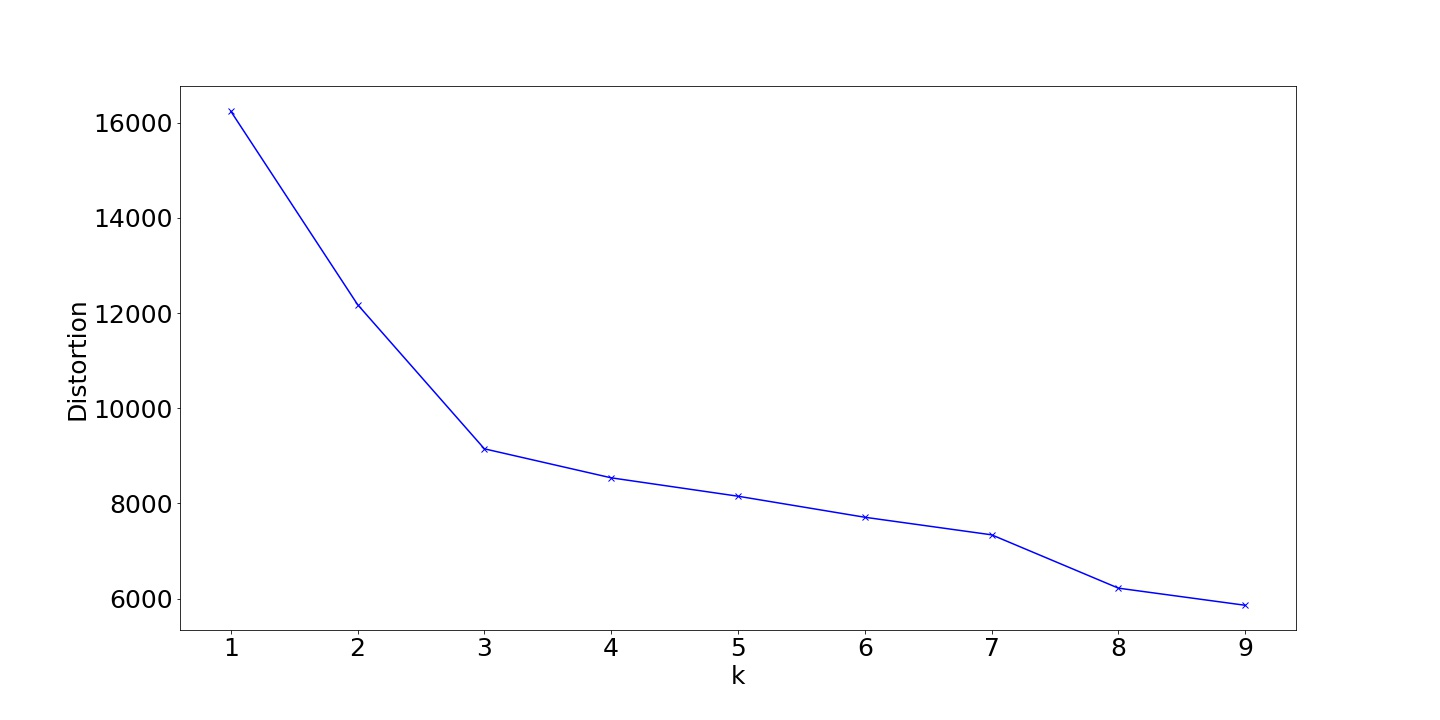
\includegraphics[width=\linewidth]{chapter3/figure/elbow.jpg}
	\caption{The Elbow Method showing the optimal k}
	\label{fig:elbow}
\end{figure}

As the clustering was completed, we inspected manually the resulting clusters.

\begin{center}
	\begin{tabular}{cc}
	\\cluster&size\\
	\hline\hline
	cluster 1&82\\
	cluster 2&648\\
	cluster 3&2\\
	cluster 4&16\\\hline
	\end{tabular}
\end{center}

Cluster 2 contains most of the samples, while the others have less elements.
We observed the Twitter profile of all the elements belonging to cluster 1, 3, 4 and a small sample of profiles of cluster 2.\\
Unfortunately there was no correlation among accounts in the same cluster, so this technique could not have helped us neither to speed up the labeling process, nor to create useful features for a classifier.

\section{Collection}

The clustering approach did not help us, but the manual inspection of the clusters allowed us to get in touch with some existing bots, making us understand which categories of bots are most common on the social network. In particular we detected 4 main categories of bots:
\begin{itemize}
	\item[\PencilRight]NSFW bots
	\item[\PencilRight]News-spreader
	\item[\PencilRight]Spambots
	\item[\PencilRight]Fake-followers
\end{itemize}

We started with a hand-labeling of the Varol \cite{Varol}. For each account we analyzed its profile and tweets and we assigned it a label according to the categories we identified. In the case of some user seemed to be an automated account, but its behavior was not understandable, we labeled it as "other".
We also found genuine users, who had been incorrectly added to the datasert.
This task culminated with the collection of the following bots:

\begin{center}
	\begin{tabular}{cc}
		\\category&labeled account\\
		\hline\hline
		NSFW&31\\
		news-spreader&71\\
		spambots&418\\
		fake-followers&5\\
		others&63\\
		genuine&104\\\hline\\		
	\end{tabular}
\end{center}

"Others" accounts often are bots with no goal, they are experiments aimed at emulating human behavior and sometimes they was recognizable just because their description informs other users about the account's nature. 
63 users are not enough to represent a class and it was not possible to find a large list of users that acted like them, so we added all this account to the "genuine" group. Even if this choise has added some noise to our data, this allowed us to create a greater differentiation between accounts of the same class.
"NSFW" accounts are only 31 elements, anyway the problem of pornography is known on Twitter. In \cite{Varol} they clusterize users too. "These bot clusters exhibit some prominent properties: cluster C0, for example, consists of legit-looking accounts that are promoting themselves (recruiters, porn actresses, etc.)" \cite{Varol}.
These kind of account are often banned by Twitter, so it is likely that the accounts that we were not able to scrape, belonged to this category.
Therefore we firmly believed that obtaining further accounts of this class was fundamental.
Finally it is clear that even fake-followers are few, since they were not considered in the Varol research, but they are important in \cite{Cresci}, so we decided to expand this category too.\\
All these data was not enough to train a classifier, hence we needed to collect more data. We perform this task by focusing on one category at a time.

\subsection{NSFW}

\subsection{News-spreader}
\subsection{Spam-bots}
\subsection{Fake-followers}
\subsection{Genuine}